\documentclass[journal]{IEEEtran}
\usepackage[T1]{fontenc}
\usepackage{amsmath,amssymb,amsfonts}
\usepackage{graphicx}
\usepackage{booktabs}
\usepackage{multirow}
\usepackage{array}
\usepackage{xcolor}
\usepackage{cite}
\usepackage{url}
\usepackage{algorithmic}
\usepackage{algorithm}
\usepackage{balance}
\graphicspath{{figures/}}
\newcommand{\dn}{\textsc{DelegNet}}

\begin{document}

\title{DelegNet: Canonical Code-Pattern Recognition for Robust, Pre-Signature Detection of Malicious EIP-7702 Delegations}

\author{Kavya and Collaborators% <-- replace with full author list and affiliations
\thanks{Manuscript prepared for submission to the IEEE Transactions on Information Forensics and Security.}}

\markboth{IEEE Transactions on Information Forensics and Security}{DelegNet: Robust Detection of Malicious EIP-7702 Delegations}

\maketitle

\begin{abstract}
EIP-7702, activated on Ethereum in May 2025, allows an externally owned account to hand its execution logic to an arbitrary smart contract with a single signed authorization. Within weeks the mechanism became the dominant vehicle for automated wallet theft: compromised and phished accounts are delegated to \emph{sweeper} and \emph{drainer} contracts that forward every incoming asset to an attacker. We present the first learning-based study of this threat. First, we construct and release a real-world dataset of $637{,}846$ EIP-7702 authorizations covering $464{,}178$ accounts and $661$ delegate contracts during the first two months after activation, with contract labels derived from observed theft outcomes rather than from the features any detector consumes. Second, we introduce a zero-day evaluation protocol in which entire families of contracts are withheld from training, and show that the industry-standard blocklist degrades to chance level ($\mathrm{AUROC}=0.500$) on unseen families. Third, we propose \dn{}, a pattern-recognition framework whose core is a \emph{canonical code-pattern recogniser}: a reachability-based canonicalisation of contract bytecode that removes, by construction, the obfuscations attackers apply to copied sweepers, combined with interpretable theft idioms and retrieval against a family-exclusive memory of known scam and benign code patterns that also serves as case-based explanation. Behaviour-centred temporal graph networks achieve the highest accuracy on non-adversarial data (AUROC $0.999$), yet we show that they are trivially evadable: when an attacker submits authorizations from the victim's own account and re-deploys disguised bytecode, their recall at a 1\% false-positive rate collapses to $0.23$. Prior-art fuzzy hashing collapses to $0.33$ under bytecode mutation. \dn{} retains a recall of $0.984$ under every attack in a five-attack adaptive-adversary suite, achieves the best first-victim detection ($\mathrm{AUROC}=0.946$), and is the only detector that screens authorizations \emph{before signing} with both high recall ($0.984$) and a negligible false-alarm rate ($0.16\%$). A label-permutation audit, class-balanced shuffled-label retraining, contract-level bootstrap intervals and equal-budget hyperparameter tuning support the validity of these findings.
\end{abstract}

\begin{IEEEkeywords}
Blockchain security, EIP-7702, account abstraction, phishing, wallet drainers, smart-contract bytecode, code canonicalisation, temporal graph neural networks, adversarial robustness, zero-day detection.
\end{IEEEkeywords}

\section{Introduction}
\label{sec:intro}

\IEEEPARstart{O}{n} 7 May 2025 the Pectra upgrade activated EIP-7702 on Ethereum mainnet~\cite{eip7702}. The proposal lets an externally owned account (EOA)---an account controlled by a single private key---publish an \emph{authorization} that designates a contract whose code is executed whenever the account is called. The feature was introduced to bring batched transactions, sponsored fees, spending limits and recovery to ordinary wallets without migrating funds. It also created an attack primitive of unusual power: one signature hands persistent, unconditional control of an account to code of the signer's choosing, and that control survives until the delegation is explicitly replaced~\cite{qi2025eip7702phishing}.

Attackers adopted the primitive within days. Industry analyses of the first weeks after activation reported that the large majority of all delegations pointed to copy-pasted contracts that automatically forward incoming ether to an attacker-controlled address~\cite{wintermute2025}. Two operational patterns dominate. In \emph{sweeping}, an attacker who already holds leaked private keys delegates thousands of victim accounts---frequently inside a single sponsored transaction---to a contract whose fallback function forwards every incoming deposit within the same transaction. In \emph{draining}, a phishing interface induces a victim to sign an authorization, after which the attacker invokes the delegated code to transfer every asset. Our dataset (Section~\ref{sec:data}) shows that $67.7\%$ of observed thefts occur in the same block as the authorization itself.

\subsection{Why existing defences are insufficient}
Deployed defences are predominantly \emph{blocklists}: wallets and explorers flag contract addresses or bytecode hashes that have already been reported. Because sweeper contracts are trivially re-deployed with a new owner address or minor bytecode edits, a blocklist cannot recognise a new family before it has claimed victims. Academic work on blockchain fraud has advanced rapidly with graph neural networks (GNNs)~\cite{weber2019aml,wu2022phishers,li2022ttagn}, but this line of work (i)~predates EIP-7702 and does not model delegation, (ii)~is typically evaluated on random or temporal splits in which test contracts or their clones appear in training, and (iii)~relies on behavioural evidence---transaction structure, timing, counterparties---that an attacker controls. Measurement studies of EIP-7702~\cite{qi2025eip7702phishing,wintermute2025,huang2026eip7702} characterise the threat with rules and static analysis but do not provide learning-based detectors or an adversarial evaluation.

\subsection{Approach and findings}
We study detection of malicious delegations under three conditions that a deployed defence actually faces: the contract family has never been seen before (\emph{zero-day}); the attacker adapts the behaviour a detector observes (\emph{adaptive evasion}); and the decision must be made \emph{before} the authorization is signed, because most thefts complete in the authorization's own block (\emph{pre-signature screening}).

We make the following observations. Temporal GNNs such as TGAT~\cite{xu2020tgat} and GraphSAGE~\cite{hamilton2017graphsage} are the most accurate detectors on non-adversarial zero-day data, but their accuracy rests on behavioural regularities of current campaigns: sponsored batch submission and repeated drains into shared sinks. When an attacker simply submits authorizations from the victim's own account, their recall at a fixed 1\% false-positive rate falls from $1.00$ to between $0.45$ and $0.55$; combining this with fresh contracts and disguised bytecode reduces it to $0.23$. Code-based detection is immune to behavioural manipulation, but the prior-art representation---fuzzy hashing of raw bytecode~\cite{kornblum2006ssdeep}---is defeated by semantics-preserving mutation, falling to a recall of $0.33$.

\dn{} resolves this tension. Its core contribution is a canonical representation of delegate bytecode that eliminates the specific transformations attackers use to evade code matching: dead and unreachable code, stack-neutral junk instruction sequences, equivalent opcode substitutions and re-laid-out jump targets. On our dataset, the four-gram similarity between an original contract and its mutated copy decays from $0.77$ to $0.19$ for raw opcodes as mutation strength increases, while the canonical form stays at $0.999$. Combined with retrieval against a memory of known patterns, from which the queried contract's own family is always excluded, the resulting recogniser holds a recall of $0.984$ under all five attacks of our adaptive-adversary suite and screens authorizations at signing time with $0.984$ recall at $0.16\%$ false alarms.

\subsection{Contributions}
\begin{enumerate}
\item \textbf{Dataset.} The first labelled real-world dataset of EIP-7702 authorizations: $637{,}846$ authorizations, $464{,}178$ accounts, $661$ delegate contracts, with recovered signers, contract bytecode, account transfer histories and outcome-derived labels with explicit evidence. Labels are derived from post-delegation theft outcomes and are therefore independent of the inputs any detector receives at decision time (Section~\ref{sec:data}).
\item \textbf{Evaluation methodology.} A zero-day protocol that withholds whole code families, evidence-history slicing that isolates a contract's first victim, a five-attack adaptive-adversary suite, a pre-signature setting, and a validity audit consisting of label-permutation tests, class-balanced shuffled-label retraining, contract-level bootstrap intervals and equal-budget tuning (Section~\ref{sec:setup}).
\item \textbf{Method.} \dn{}, a pattern-recognition framework comprising a canonical code representation with a constructive invariance argument, interpretable theft idioms, and a family-exclusive code-pattern memory whose nearest matches double as case-based explanations (Section~\ref{sec:method}).
\item \textbf{Findings.} Behavioural graph detectors are accurate on non-adversarial data but evadable; raw code matching is evadable by mutation; canonical code-pattern recognition is the only approach that is simultaneously robust to behavioural evasion, robust to code disguise, and usable before signing (Section~\ref{sec:results}).
\end{enumerate}

\section{Background and Threat Model}
\label{sec:background}

\subsection{EIP-7702 delegation}
An EIP-7702 transaction (type~\texttt{0x04}) carries an \emph{authorization list}. Each entry is a tuple $(\chi, a, n, y, r, s)$ of a chain identifier $\chi$, a delegate address $a$, the signer's nonce $n$ and a secp256k1 signature. The signer---the \emph{authority}---is not transmitted; it is recovered from the signature over $\mathrm{keccak}(\mathtt{0x05}\,\|\,\mathrm{rlp}(\chi, a, n))$. Processing an entry sets the authority's code to the designator $\mathtt{0xef0100}\,\|\,a$, after which any call to the authority executes $a$'s code in the authority's context, with full access to its balance and token approvals. Three properties matter for security:
\begin{itemize}
\item The transaction may be submitted by any account (the \emph{sponsor}), so the signer need not hold ether for fees.
\item A single transaction may carry many authorizations, enabling bulk delegation.
\item Authorizations are applied before the transaction's call executes, so a sponsor can delegate a victim and invoke the delegated code atomically.
\end{itemize}

\subsection{Attack patterns}
We distinguish two families of malicious delegate contracts, observed throughout our data.
\paragraph{Sweepers} The fallback function forwards the full balance to a hard-coded address whenever value arrives. An attacker holding leaked keys delegates victims in bulk; every subsequent deposit---including deposits made by victims attempting recovery, or by unwitting payers---is forwarded within the depositing transaction.
\paragraph{Drainers} An owner-gated entry point (for example an \texttt{execute} function guarded by a comparison of the caller with a hard-coded attacker address) lets the attacker issue arbitrary calls from the victim's account, emptying ether and tokens. Delegation is obtained through phishing.

Benign delegates include smart-account implementations whose entry points are guarded by a signature check against the account itself or by a self-call requirement, batch executors, session-key wallets and account-abstraction wallets. Some benign contracts---for example auto-forwarders that send deposits to the user's own cold wallet---are structurally close to sweepers, which makes pure syntactic signatures unreliable.

\subsection{Threat model}
We consider an attacker who controls (i)~which account submits an authorization, (ii)~whether authorizations are batched, (iii)~whether a fresh sponsor account and a freshly deployed contract are used for each victim, and (iv)~the bytecode of the delegate, subject to preserving its malicious semantics. The attacker cannot change the semantics their contract must have in order to steal (forwarding value to attacker-controlled destinations, or granting an attacker-controlled caller arbitrary execution). The defender observes the chain up to a decision time, which may be before the authorization is included (pre-signature screening by a wallet), at its inclusion, or later. The defender is assumed to have labelled examples of earlier contract families but none of the family being evaluated.

\section{Related Work}
\label{sec:related}

\paragraph{Graph learning for blockchain fraud} Weber \emph{et al.}~\cite{weber2019aml} introduced graph convolutional networks~\cite{kipf2017gcn} for anti-money-laundering on Bitcoin. On Ethereum, phishing-account detection has progressed from network embeddings~\cite{wu2022phishers} to temporal aggregation~\cite{li2022ttagn} and temporal graph networks~\cite{xu2020tgat,rossi2020tgn}, with reported AUROCs close to $1.0$. These methods learn behavioural patterns of accounts. They are evaluated on random or temporal splits in which the same scam contracts recur between training and test, and they are not assessed against attackers who change the observable behaviour. Our results show that both factors substantially overstate deployed performance for EIP-7702 attacks.

\paragraph{Smart-contract fraud and code analysis} Ponzi-scheme and honeypot detection used opcode statistics and symbolic analysis of contract code~\cite{chen2018ponzi,torres2019honeybadger}. Code-similarity approaches, including context-triggered piecewise hashing~\cite{kornblum2006ssdeep} and learned code embeddings~\cite{gao2019smartembed}, are effective for clone detection but are sensitive to syntactic perturbation. Our canonicalisation is related to normalisation in binary similarity analysis; we tailor it to the EVM's stack semantics and to the transformations that occur in practice when sweeper code is copied.

\paragraph{MEV and transaction ordering} Front-running and miner-extractable value have been characterised extensively~\cite{daian2020flashboys,torres2021frontrunner}. These works analyse attacks against transactions rather than against account control, but they motivate our attention to atomic, same-block behaviour.

\paragraph{EIP-7702 security} Concurrent measurement work quantifies malicious delegation shares and identifies sweeper families with rules and static analysis~\cite{wintermute2025,huang2026eip7702}. Qi \emph{et al.}~\cite{qi2025eip7702phishing} analyse phishing paths to account takeover. None proposes a learned detector, a zero-day evaluation or an adversarial evaluation.

\paragraph{Robustness and interpretability} Adversarial attacks on graph learners perturb graph structure or node features under a budget~\cite{zugner2018nettack}. In our setting the attacker's leverage is behavioural and economically negligible: choosing who submits an authorization or deploying a fresh contract costs a few transactions. We model these levers explicitly rather than as abstract perturbation budgets. For interpretability, prototype reasoning~\cite{chen2019thislooks} and post-hoc explainers such as GNNExplainer~\cite{ying2019gnnexplainer} justify decisions through learned exemplars or important substructures. \dn{} is case-based by construction: every decision is justified by the specific previously observed contract it matches, which an analyst can inspect on chain. Temporal network motifs~\cite{paranjape2017motifs} inform the behavioural features we provide to the baselines.

Table~\ref{tab:related} summarises how our study differs from prior work.

\begin{table}[t]
\centering
\caption{Positioning against prior work. \checkmark: addressed; --: not addressed.}
\label{tab:related}
\setlength{\tabcolsep}{3pt}
\footnotesize
\begin{tabular}{lcccccc}
\toprule
Work & 7702 & Learned & Zero-day & Adaptive & Pre-sign. & Data \\
\midrule
GCN AML~\cite{weber2019aml} & -- & \checkmark & -- & -- & -- & \checkmark \\
Phishing GNNs~\cite{wu2022phishers,li2022ttagn} & -- & \checkmark & -- & -- & -- & -- \\
Fuzzy hashing~\cite{kornblum2006ssdeep} & -- & -- & partial & -- & \checkmark & -- \\
7702 measurement~\cite{wintermute2025,huang2026eip7702} & \checkmark & -- & -- & -- & -- & partial \\
7702 phishing~\cite{qi2025eip7702phishing} & \checkmark & -- & -- & -- & -- & -- \\
\textbf{This work} & \checkmark & \checkmark & \checkmark & \checkmark & \checkmark & \checkmark \\
\bottomrule
\end{tabular}
\end{table}

\section{Dataset Construction}
\label{sec:data}

No public dataset of EIP-7702 attacks existed when this study began, and existing blockchain-fraud corpora predate the mechanism. We therefore built a dataset directly from the Ethereum ledger. This section describes collection, signer recovery, sampling, outcome-based labelling and the validation of those labels. The design goal throughout was that labels must be derived from information that no detector can observe at its decision time.

\subsection{Collection}
\paragraph{Window} We collected all blocks from the Pectra activation block ($22{,}431{,}084$, 7~May~2025) to block $22{,}863{,}596$ (7~July~2025), a window of $432{,}513$ blocks. The first two months contain the initial adoption of the mechanism by both legitimate wallets and attackers, including the large sweeper campaigns reported by industry~\cite{wintermute2025}.

\paragraph{Authorization scan} Every block was retrieved with full transaction bodies, and every type-\texttt{0x04} transaction was expanded into its authorization tuples. Because the signer of an authorization is not part of the transaction, we recovered it from the secp256k1 signature over the EIP-7702 message digest. To validate recovery, we sampled recovered authorities and compared their current on-chain code with the expected designator $\mathtt{0xef0100}\,\|\,a$; every sampled authority matched. Tuples whose chain identifier was neither $0$ nor $1$, and $21$ tuples with invalid signatures ($0.003\%$), were discarded, as the protocol itself rejects them.

\paragraph{Contract code} For every delegate address we retrieved the deployed bytecode, yielding $661$ distinct delegate contracts.

\paragraph{Account activity} To characterise what happens after a delegation, we collected the value transfers of the accounts involved: every top-level and internal ether transfer that sends value from or to a tracked account, obtained through transaction-trace filtering. Internal transfers are essential, because a sweeper moves funds inside the depositing transaction rather than through a transaction of its own. For each transfer that leaves an authority, we additionally retrieved the sender of the enclosing transaction. This distinguishes outflows initiated by the account owner from outflows triggered by a third party through the delegated code. A second hop collected the activity of candidate attacker sinks---recipients of third-party-triggered outflows---and of the accounts that funded sponsors.

\paragraph{Sampling} Collecting the transfer histories of all $464{,}178$ authorities through public endpoints was infeasible, because the largest sweeper campaigns alone delegated more than $100{,}000$ accounts to a single contract. We applied stratified sampling: every authorization of contracts with at most $1{,}000$ delegators was retained, and $1{,}000$ delegators were drawn uniformly over time for larger contracts. All authorizations made by a sampled authority were kept, so that its delegation history is complete. The working set comprises $165{,}846$ authorizations by $22{,}501$ authorities across all $661$ contracts. Sampling is per contract and uniform in time, so per-contract delegation dynamics are preserved, while the dominance of a handful of mega-campaigns---which would otherwise make any metric an evaluation of those campaigns alone---is reduced.

\subsection{Outcome-based labelling}
A delegation is labelled through its delegate contract. For each contract we aggregate what happened to the accounts that delegated to it, using only outflows from an authority that occur while its delegation is in force and within $24$ hours of it. For each such outflow we record whether it was triggered by a third party (the enclosing transaction was sent by an account other than the authority) and whether its recipient is an externally owned account. A recipient that receives third-party-triggered outflows from at least two distinct authorities of the same contract is a \emph{shared sink}. From these observations we compute, per contract: the number of drained authorities; the drained ratio; the share of drained authorities that drained into shared sinks; the share of all third-party outflow events that terminate in shared sinks; and the share of authorities that continued to initiate their own outflows after delegating (\emph{self-activity}). Table~\ref{tab:labels} lists the decision rules.

\begin{table}[t]
\centering
\caption{Outcome-based contract labelling rules. Contracts meeting neither rule remain unlabelled and are excluded from supervised evaluation.}
\label{tab:labels}
\footnotesize
\setlength{\tabcolsep}{4pt}
\begin{tabular}{p{0.32\columnwidth}p{0.58\columnwidth}}
\toprule
Label & Conditions (all must hold) \\
\midrule
Malicious & $\ge 3$ drained authorities; drained ratio $\ge 0.02$; $\ge 60\%$ of drained authorities drained into shared sinks; $\ge 80\%$ of third-party outflow events end in shared sinks; owner self-activity $\le 20\%$ \\
Benign & $\ge 5$ authorities; drained ratio $\le 0.05$; owner self-activity $\ge 30\%$ \\
\bottomrule
\end{tabular}
\end{table}

The rules encode the operational signature of theft rather than any property a detector uses. A sweeper's victims lose deposits to the same few attacker accounts, the outflows are triggered by whoever sent the deposit rather than by the owner, and owners stop using the account; a benign smart-account implementation shows owners transacting normally and no concentration of value into third-party sinks. Two design choices deserve justification. First, the drained-ratio threshold is deliberately low. A sweeper fires only when funds arrive, and most leaked-key accounts are empty: the largest sweeper in our window, with $968$ delegators in the first week, had drained only $7\%$ of them while concentrating $100\%$ of third-party outflows into shared sinks with $0\%$ owner self-activity. A majority-drained requirement would have labelled it benign. Second, we do not exclude outflows whose recipient equals the transaction sender. In the dominant sweeper pattern the attacker is simultaneously the sponsor, the sender of the draining transaction and its recipient; excluding self-addressed outflows, a natural filter for relayer fees, removed every drain of the largest campaign during development. Relayer fees are instead excluded by the concentration requirement, as they are small and dispersed.

\paragraph{Separation of labels and inputs} Labels depend on outflows that occur \emph{after} each delegation. A detector at decision time $t$ observes only events up to $t$. For evaluation at the moment of authorization, the target's own drains are therefore never visible. Information about \emph{earlier} delegators of the same contract is legitimately visible to a deployed detector and is used by some models; Section~\ref{sec:setup} explains how our evaluation isolates its effect.

\paragraph{Independent cross-check} We matched contracts, their sponsors and their drain sinks against a public scam-address list~\cite{scamsniffer}. No benign contract was linked to a listed address. The list focuses on phishing websites rather than leaked-key sweeping, and none of the malicious contracts' operators appeared on it---an observation that itself illustrates the coverage gap of list-based defences.

\subsection{Statistics}
Table~\ref{tab:stats} summarises the dataset and Fig.~\ref{fig:dataset} characterises it. Delegation volume is dominated by a few campaigns: the delegator distribution per contract is heavy-tailed, and malicious contracts reach tens of thousands of delegators. $67.6\%$ of authorizations are submitted in batches containing more than one authorization, a hallmark of sponsored campaigns. Thefts are almost instantaneous: $67.7\%$ occur in the same block as the authorization and the median delay is zero seconds, because sponsors delegate and invoke the delegated code atomically. This single observation drives a key design requirement: a defence that acts after an authorization is included cannot prevent most thefts.

\begin{table}[t]
\centering
\caption{Dataset statistics (Ethereum, 7 May -- 7 July 2025).}
\label{tab:stats}
\footnotesize
\begin{tabular}{lr}
\toprule
Quantity & Value \\
\midrule
Authorizations (all) & 637{,}846 \\
\quad non-revoking & 634{,}828 \\
Authorities (distinct accounts) & 464{,}178 \\
Sponsors (distinct submitters) & 63{,}951 \\
Delegate contracts & 661 \\
Authorizations in multi-authorization batches & 67.6\% \\
Working set: authorizations / authorities & 165{,}846 / 22{,}501 \\
Temporal graph: nodes / events & 443{,}800 / 4{,}792{,}530 \\
Distinct (authority, contract) targets & 36{,}473 \\
\quad malicious / benign / unlabelled & 11{,}320 / 3{,}201 / 21{,}952 \\
Labelled contracts: malicious / benign & 49 / 11 \\
Code families (all / labelled) & 334 / 41 \\
\quad labelled families: malicious / benign & 32 / 9 \\
Attack campaigns (connected components) & 30 \\
Thefts in the authorization's block & 67.7\% \\
Median authorization-to-theft delay & 0 s \\
\bottomrule
\end{tabular}
\end{table}

\begin{figure}[t]
\centering
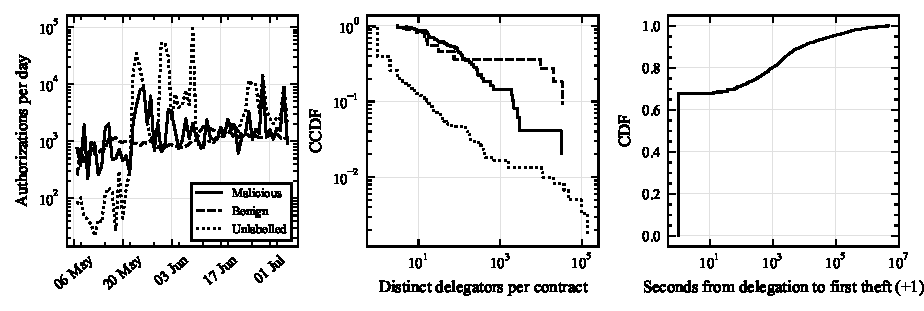
\includegraphics[width=0.4\textwidth]{fig_dataset}
\caption{Dataset characterisation. Left: daily authorizations by contract label (log scale); sweeper campaigns produce bursts of tens of thousands of authorizations per day. Centre: complementary cumulative distribution of distinct delegators per contract; malicious contracts dominate the heavy tail. Right: cumulative distribution of the delay from authorization to first theft; two thirds of thefts occur in the same block.}
\label{fig:dataset}
\end{figure}

\paragraph{Targets} A sweeper often re-authorizes the same victim repeatedly. To prevent near-duplicate examples from appearing on both sides of a split, the prediction target is the first authorization of each (authority, contract) pair, yielding $36{,}473$ targets, of which $14{,}521$ belong to labelled contracts.

\paragraph{Code families} Copy-pasted contracts differ in hard-coded addresses and minor edits, so contract identity is too fine a unit for generalisation tests. We group contracts into \emph{code families} by canonical opcode four-gram Jaccard similarity of at least $0.8$ (Section~\ref{sec:method}), using union-find over exact canonical duplicates first. This yields $334$ families, $41$ of them labelled ($32$ malicious, $9$ benign). The scarcity of benign families---the consequence of requiring at least five delegators and sustained owner activity---is the dataset's principal limitation and recurs in our analysis of learned model combination (Section~\ref{sec:discussion}).

\paragraph{Campaigns} For attribution analysis, malicious delegations are connected when they share a delegate contract, a sponsor or a first drain sink; connected components define $30$ campaigns. Campaign identifiers are used only to score attribution, never as model inputs.

\section{DelegNet}
\label{sec:method}

\subsection{Problem formulation}
A delegation event $e=(u,s,c,t)$ records that authority $u$ delegated to contract $c$ through a transaction submitted by sponsor $s$ at time $t$. Let $\mathcal{H}_{\tau}$ denote all chain events observable up to a decision time $\tau$. A detector is a function $f(e,\mathcal{H}_{\tau}) \in [0,1]$ estimating the probability that $c$ is malicious. We consider three decision times:
\begin{itemize}
\item \emph{pre-signature}, $\tau=t^-$: the authorization is not yet on chain and the sponsor is unknown, which is the situation of a wallet asked to sign;
\item \emph{inclusion}, $\tau=t$: the authorization and its transaction are visible;
\item \emph{monitoring}, $\tau=t+\delta$, $\delta\in\{12,60,300,1800,7200\}$\,s.
\end{itemize}
The defender's training data contain labelled contracts from code families $\mathcal{F}_{\mathrm{train}}$, and evaluation contracts come from disjoint families $\mathcal{F}_{\mathrm{test}}$, $\mathcal{F}_{\mathrm{train}}\cap\mathcal{F}_{\mathrm{test}}=\emptyset$.

\subsection{Design rationale}
Two observations drive the design. First, the semantics that a theft requires---forwarding the account's value to attacker-controlled destinations, or granting an attacker-controlled caller arbitrary execution---must be present in the delegate's code, whereas the behavioural context of a delegation (who submits it, in what batch, from which funding source, how long before the drain) is chosen freely and cheaply by the attacker. A detector whose decision rests on code semantics therefore resists the cheapest evasions. Second, attackers mass-produce their contracts by copying, and the copies differ by exactly the edits that defeat syntactic matching: new hard-coded addresses, junk instructions, equivalent instruction choices and appended data. A representation that is invariant to those edits, but preserves what the code does, turns copy-paste into a liability for the attacker rather than an evasion.

\dn{} is organised as a pattern-recognition module with three stages: (A)~a canonical code representation that removes attacker-controlled syntactic variation, (B)~interpretable theft idioms computed on that representation, and (C)~a family-exclusive memory of known scam and benign code patterns that produces the detection score and, through its nearest match, a case-based explanation.

\subsection{Canonical code representation}
\label{sec:canon}
Delegate contracts execute on the Ethereum Virtual Machine (EVM), a stack machine whose bytecode interleaves single-byte opcodes and immediate operands (\texttt{PUSH1}--\texttt{PUSH32} carry 1--32 operand bytes). Control flow uses \texttt{JUMP}/\texttt{JUMPI} to absolute byte offsets that must hold a \texttt{JUMPDEST} instruction. Our canonicalisation maps bytecode $b$ to a token sequence $\kappa(b)$ in five steps.

\paragraph{Step 1: disassembly and code-address identification} The bytecode is decoded into instructions $(o_i,v_i,\pi_i)$ with opcode $o_i$, immediate $v_i$ and byte offset $\pi_i$. Undefined bytes are kept verbatim as \texttt{INVALID} with their raw value, so that decoding and re-encoding are lossless. We identify immediates that encode code addresses: a push whose value equals the offset of a \texttt{JUMPDEST} and is immediately followed by a jump (a static jump), or a push of at least two bytes whose value equals a \texttt{JUMPDEST} offset (a return address pushed for an internal call, the pattern Solidity emits for function calls). One-byte pushes are tagged only if their value is not a common memory or calldata constant (multiples of 32 and the calldata argument offsets $4+32k$), because those values coincide with low code offsets in small contracts.

\paragraph{Step 2: reachability} Starting from offset $0$, we compute the set of reachable instructions by a worklist closure. Execution falls through until a terminator (\texttt{STOP}, \texttt{RETURN}, \texttt{REVERT}, \texttt{INVALID}, \texttt{SELFDESTRUCT}, \texttt{JUMP}), and every \texttt{JUMPDEST} whose offset is pushed by a reachable instruction becomes a new root. Unreachable instructions---compiler metadata, appended data and attacker-appended padding---are dropped.

\paragraph{Step 3: equivalence normalisation} Instruction sequences with identical effect on the stack and state are rewritten to one representative: \texttt{ADDRESS BALANCE}$\,\to\,$\texttt{SELFBALANCE}; \texttt{XOR ISZERO}$\,\to\,$\texttt{EQ} (since $a=b \Leftrightarrow (a \oplus b)=0$); \texttt{PUSH1 0x00}$\,\to\,$\texttt{PUSH0}.

\paragraph{Step 4: junk elimination} A peephole pass removes, to a fixed point, sequences whose net effect on the stack is empty and which have no side effect: a push followed by \texttt{POP}; an environment read (\texttt{GAS}, \texttt{CALLVALUE}, \texttt{PC}, \texttt{MSIZE}, \texttt{ADDRESS}, \texttt{CALLER}, \texttt{CALLDATASIZE}, \texttt{RETURNDATASIZE}) followed by \texttt{POP}; \texttt{PUSH0 ISZERO POP}; and \texttt{PUSH}$\,$\texttt{PUSH}$\,$\texttt{SWAP1}$\,$\texttt{POP}$\,$\texttt{POP}. \texttt{JUMPDEST} markers are removed entirely, because their positions are precisely what instruction insertion shifts, while the control-flow information they carry is preserved by Step~5.

\paragraph{Step 5: semantic tagging} Pushed code addresses and all two- and three-byte pushes become a single \texttt{TAG} token, so that re-laid-out jump targets compare equal. Four-byte pushes equal to well-known function selectors (ERC-20 \texttt{transfer}, \texttt{transferFrom}, \texttt{approve}, \texttt{setApprovalForAll}, \texttt{permit}, Permit2, ERC-1271 \texttt{isValidSignature}, ERC-4337 \texttt{validateUserOp}, \texttt{execute} variants, proxy upgrades, token-receiver hooks) become named tokens. Twenty-byte pushes become \texttt{ADDR}, so that copies with different hard-coded owners compare equal. Small constants in $[1,10]$---including precompile addresses such as \texttt{ecrecover}---are tagged by push width. All other opcodes are kept.

\begin{algorithm}[t]
\caption{Canonicalisation $\kappa(b)$ of EVM bytecode}
\label{alg:canon}
\begin{algorithmic}[1]
\REQUIRE bytecode $b$
\STATE $I \leftarrow$ decode$(b)$ \COMMENT{lossless; undefined bytes kept}
\STATE $D \leftarrow \{\pi_i : o_i=\texttt{JUMPDEST}\}$
\STATE mark $i$ as code-address push if $v_i\in D$ and ($o_{i+1}\in\{\texttt{JUMP},\texttt{JUMPI}\}$ or width $\ge 2$ or $v_i\notin C_{\text{common}}$)
\STATE $R \leftarrow \emptyset$; $Q \leftarrow \{0\}$ \COMMENT{reachability}
\WHILE{$Q\neq\emptyset$}
\STATE pop $k$; \textbf{while} $k\notin R$: add $k$ to $R$; push target of any reachable code-address push onto $Q$; \textbf{break} at terminator; $k\leftarrow k+1$
\ENDWHILE
\STATE $I \leftarrow [\,i\in I : i\in R\,]$
\STATE rewrite equivalences: \texttt{ADDRESS BALANCE}$\to$\texttt{SELFBALANCE}, \texttt{XOR ISZERO}$\to$\texttt{EQ}, \texttt{PUSH1 0}$\to$\texttt{PUSH0}
\STATE drop \texttt{JUMPDEST}; remove stack-neutral suffixes ending in \texttt{POP} to a fixed point
\STATE map: code-address and 2--3-byte pushes $\to$ \texttt{TAG}; 20-byte pushes $\to$ \texttt{ADDR}; known selectors $\to$ names; small constants $\to$ width tags
\RETURN token sequence
\end{algorithmic}
\end{algorithm}

\begin{table}[t]
\centering
\caption{Worked example: the forwarding core of a sweeper, a disguised copy, and their common canonical form. Junk (italic) and equivalent substitutions (underlined) are removed or normalised.}
\label{tab:canon-example}
\footnotesize
\setlength{\tabcolsep}{2pt}
\begin{tabular}{p{0.3\columnwidth}p{0.36\columnwidth}p{0.26\columnwidth}}
\toprule
Original & Disguised copy & Canonical \\
\midrule
\texttt{PUSH0} & \texttt{PUSH1 0x00} & \texttt{PUSH0} \\
\texttt{PUSH0 PUSH0 PUSH0} & \emph{\texttt{GAS POP}} \texttt{PUSH0 PUSH0 PUSH0} & \texttt{PUSH0 PUSH0 PUSH0} \\
\texttt{SELFBALANCE} & \underline{\texttt{ADDRESS BALANCE}} & \texttt{SELFBALANCE} \\
\texttt{PUSH20 0xA1\ldots} & \texttt{PUSH20 0x7C\ldots} (new owner) & \texttt{ADDR} \\
\texttt{GAS CALL POP} & \emph{\texttt{PUSH2 0x3f1 PUSH1 9 SWAP1 POP POP}} \texttt{GAS CALL POP} & \texttt{GAS CALL POP} \\
\texttt{STOP} & \texttt{STOP} \emph{\texttt{INVALID 0x5b\ldots}} (trailer) & \texttt{STOP} \\
\bottomrule
\end{tabular}
\end{table}

Algorithm~\ref{alg:canon} summarises the procedure and Table~\ref{tab:canon-example} illustrates it on the forwarding core shared by most sweepers in our data. Raw four-gram similarity between the two left columns is low---every inserted instruction breaks several four-grams---whereas their canonical sequences are identical. The idiom ``\texttt{SELFBALANCE} feeding a \texttt{CALL} to a hard-coded address'' survives intact.

\paragraph{Invariance} Let $\mathcal{M}$ be the set of mutations that (i)~insert a stack-neutral sequence from the set $\mathcal{N}$ eliminated in Step~4 at any instruction boundary other than between a static push and its jump, (ii)~apply a rewrite from Step~3 in either direction, (iii)~append an unreachable trailer, and (iv)~re-encode code-address immediates to the new offsets, possibly widening the push. For any $b$ and $m\in\mathcal{M}^{*}$ that preserves the reachable control-flow graph, $\kappa(m(b))=\kappa(b)$. The argument is constructive. Trailers are unreachable and removed by Step~2. Inserted $\mathcal{N}$-sequences are reachable but eliminated by Step~4, whose rules are confluent because each rule removes a contiguous suffix ending in \texttt{POP} and introduces no new instructions. Rewrites from Step~3 map to the same representative. Re-encoded code addresses become \texttt{TAG} irrespective of value and width, and \texttt{JUMPDEST} tokens are removed, so offset shifts are invisible. Equality fails only when a mutation creates a sequence outside $\mathcal{N}$ or alters the reachable control flow, which by definition changes the program. Empirically, over $60$ malicious contracts and six mutation strengths, the canonical four-gram similarity between a contract and its mutated copy is $0.999$ on average, against $0.192$--$0.766$ for raw opcodes (Section~\ref{sec:res-disguise}).

\paragraph{Mutation engine} To evaluate and train against disguise we implemented a semantics-preserving mutator over disassembled code. It inserts stack-neutral sequences with probability $\min(0.5,0.06\,\sigma)$ per instruction, substitutes equivalent forms with probability $\min(0.9,0.25\,\sigma)$, appends an unreachable trailer of up to $24\sigma$ bytes, and re-links all identified code addresses, iteratively widening pushes until every target fits. Mutation strength $\sigma$ controls all three. Each mutant is verified: its reachable instruction count must not decrease, otherwise it is regenerated (after five failures the mutator falls back to substitution only). This guarantees that evaluation uses only mutants whose control flow survives.

\subsection{Code idioms}
From $\kappa(b)$ we compute $21$ interpretable indicators of theft-relevant semantics:
\begin{itemize}
\item value forwarding: a \texttt{CALL} preceded within twelve instructions by \texttt{SELFBALANCE}, and specifically to a hard-coded \texttt{ADDR};
\item caller authorisation: \texttt{CALLER} compared with a hard-coded address (owner gate) or with \texttt{ADDRESS} (self-call gate);
\item \texttt{ORIGIN} use;
\item signature verification: a \texttt{STATICCALL} to the \texttt{ecrecover} precompile;
\item \texttt{DELEGATECALL} in general, and to a calldata- or storage-derived target;
\item \texttt{SELFDESTRUCT};
\item token-transfer, transfer-from, approval, permit, upgrade and account-abstraction selectors;
\item counts of dispatched selectors, hard-coded addresses, calls and storage writes;
\item canonical length, and whether the fallback region performs a call.
\end{itemize}
Because they are computed on $\kappa(b)$, the idioms inherit its invariance. Over all evaluated contracts, $34$--$36$ of $36$ contracts retained identical idiom vectors under mutation at every strength during development.

\subsection{Code-pattern memory and detection score}
\label{sec:memory}
Let $G(b)$ be the set of four-grams of $\kappa(b)$, and $J(A,B)=|A\cap B|/|A\cup B|$ the Jaccard similarity. From the training delegations we build a memory $\mathcal{M}=\{(F_j,G_j,\bar y_j)\}$ containing, for each training contract $j$, its code family $F_j$, four-gram set $G_j$ and mean label $\bar y_j$. For a query contract $q$ with family $F_q$ we compute
\begin{align}
\sigma_{\mathrm{mal}}(q)&=\max_{j:\,\bar y_j\ge 0.5,\;F_j\ne F_q} J\big(G(q),G_j\big),\\
\sigma_{\mathrm{ben}}(q)&=\max_{j:\,\bar y_j< 0.5,\;F_j\ne F_q} J\big(G(q),G_j\big),
\end{align}
and the detection score $f(q)=\tfrac{1}{2}\big(1+\sigma_{\mathrm{mal}}(q)-\sigma_{\mathrm{ben}}(q)\big)$. The score is a signed nearest-pattern margin: a contract that resembles known theft code more than known wallet code scores above $\tfrac12$.

The exclusion $F_j\ne F_q$ makes training-time and test-time behaviour identical. In the zero-day protocol a test family is absent from the memory by construction; excluding the query's own family whenever the memory is queried for a training contract---for example when selecting the operating threshold or analysing score distributions---prevents a contract from matching itself or its own clones with similarity $1.0$, a value genuinely new families never attain. With exclusion, the largest similarity a training contract attains in our data is $0.61$, in line with what unseen families exhibit.

The score depends only on the delegate's code. It is therefore available before signing, unaffected by who submits the authorization or how it is batched, and---through canonicalisation---unaffected by the disguises in $\mathcal{M}$. Its cost is $O(|\mathcal{M}|\,|G|)$ set operations per previously unseen contract, with results cached per canonical code.

\subsection{Case-based explanation}
Every score is accompanied by its evidence: the nearest malicious and nearest benign memory entries, their similarities, and the idioms that differ between the query and each match. Because memory entries are deployed contracts, an analyst can inspect the matched contract, its delegators and its drains directly on chain. This form of explanation is faithful by construction---the score is a function of exactly these two similarities---and does not require a post-hoc approximation of a black-box model.

\subsection{Operating point}
The decision threshold is chosen on validation families for a target false-positive rate of 1\%, computed on benign validation delegations only. Thresholds are never tuned on test data. Because the score depends on the delegate's code alone, one threshold serves every decision time: pre-signature, inclusion and monitoring.

\subsection{Complexity and deployment}
Canonicalisation is linear in code length, and the reachability closure visits each instruction at most once. Scoring a previously unseen contract costs one Jaccard computation per memory entry over sets of a few hundred four-grams; with $60$ labelled training contracts this is sub-millisecond, and results are cached per canonical code. A wallet can therefore score a delegation request locally while the user is reviewing the signature prompt, and update the memory as new families are confirmed, without retraining any model.

\section{Experimental Methodology}
\label{sec:setup}

\subsection{Baselines}
We compare \dn{} with five detectors that represent current practice and the strongest learned alternatives. All learned baselines receive strictly more information than \dn{}: the complete behavioural context of each delegation, in addition to code features.

\paragraph{Blocklist} An exact-match list: a contract is flagged if its canonical code was labelled malicious in training, cleared if it was labelled benign, and scored $0.5$ otherwise. This mirrors wallet and explorer warnings, and is in fact stronger than address- or raw-hash-based lists, because canonical matching already absorbs re-deployment with new constants.

\paragraph{Fuzzy hash} The prior-art code-similarity approach: nearest-neighbour Jaccard similarity of four-grams of the \emph{raw} opcode sequence, with the same signed-margin score as \dn{}. It isolates the contribution of canonicalisation, since memory, scoring and family exclusion are identical.

\paragraph{XGBoost} Gradient-boosted trees~\cite{chen2016xgboost} on $101$ features: $18$ running statistics for each of the authority, sponsor and contract; $21$ behavioural motif statistics; $5$ authorization features; and the $21$ code idioms of Section~\ref{sec:method}. The behavioural motifs, inspired by temporal network motifs~\cite{paranjape2017motifs}, cover campaign infrastructure (batch size, gas funding of the authority by the sponsor, sponsor breadth and age, funding of the sponsor by a known sink), sibling evidence over up to $256$ earlier delegators of the same contract (fractions drained within 24\,h or 60\,s, swept, still self-active or departed, maximal shared sink, sponsor diversity, sink fan-out) and the authority's own history. All motifs are counted exactly at the decision cutoff using chain-order event identifiers, so that a same-block drain is never visible when deciding at the authorization itself.

\paragraph{GraphSAGE and TGAT} Two temporal graph neural networks over a heterogeneous event graph whose nodes are accounts and contracts and whose events are authorizations, sponsorships, revocations and value transfers. Event features are the normalised value (log-ratio to the asset's median in the first 20\% of the window), token and internal-call flags, a flag for outflows triggered by a third party, the log batch size and self-sponsorship. Node features are $18$ statistics read at the cutoff from per-node cumulative arrays in logarithmic time. For each delegation we sample the $24$ most recent events of the authority, sponsor and contract and the $8$ most recent events of each neighbour, up to $256$ nodes, all with chain-order identifiers not exceeding the cutoff. TGAT~\cite{xu2020tgat} applies two layers of multi-head attention over messages carrying the source state, the event features and a learnable functional time encoding $\phi(\Delta t)=\cos(\omega\Delta t+\beta)$ with frequencies spanning seconds to months:
\begin{equation}
\alpha_{vw}=\operatorname{softmax}_{w\in\mathcal{N}(v)}\frac{(W_q h_v)^{\top}W_k\,[h_w\,\|\,\phi(\Delta t_{vw})\,\|\,x_{vw}]}{\sqrt{d}} .
\end{equation}
GraphSAGE~\cite{hamilton2017graphsage} replaces attention by mean aggregation and omits the time encoding. Both read out the states of the authority, sponsor and contract together with the authorization features. Both are trained with class-weighted cross-entropy and contract-balanced sampling---each (contract, class) group receives equal weight in each epoch of $6{,}000$ draws, so that mega-campaigns do not dominate---and are selected by class-balanced validation log-loss, because validation AUPRC saturates at $1.0$ within a few epochs on this task.

\subsection{Equal-budget tuning}
Every method with hyperparameters receives the same budget: six random configurations, each trained on the training families of all three zero-day folds and scored on those folds' \emph{validation} families by mean AUROC (ties broken by validation log-loss). Test families are never used. Table~\ref{tab:tuning} lists the search spaces and selected configurations. \dn{} has no learned parameters; its only choices, the four-gram order and the 1\% false-positive operating point, were fixed before evaluation.

\begin{table}[t]
\centering
\caption{Equal-budget tuning on validation families (6 trials each).}
\label{tab:tuning}
\footnotesize
\setlength{\tabcolsep}{3pt}
\begin{tabular}{lp{0.43\columnwidth}p{0.27\columnwidth}}
\toprule
Method & Search space & Selected \\
\midrule
TGAT & lr $\{10^{-3},5{\cdot}10^{-4},2{\cdot}10^{-4}\}$, width $\{64,128\}$, dropout $\{0.1,0.3\}$, layers $\{1,2\}$, weight decay $\{10^{-4},10^{-3}\}$ & $2{\cdot}10^{-4}$, 128, 0.1, 2, $10^{-3}$ \\
GraphSAGE & as TGAT & $5{\cdot}10^{-4}$, 64, 0.1, 2, $10^{-3}$ \\
XGBoost & depth $\{3,4,6,8\}$, learning rate $\{0.03,0.1\}$, min.\ child weight $\{1,5\}$, subsample $\{0.7,1.0\}$, column sample $\{0.6,0.9\}$ & 8, 0.03, 1, 1.0, 0.6 \\
\dn{} & none (non-parametric) & -- \\
\bottomrule
\end{tabular}
\end{table}

\subsection{Zero-day protocol}
Labelled code families are dealt, separately for each class, into three folds by a seeded permutation. In each fold, the families of that fold form the test set. From the remaining families, whole families covering approximately 15\% of each class form the validation set, and the rest form the training set. No contract, and no clone of a contract, appears in more than one of the three sets. Each delegation is scored exactly once per seed, by a model that has never seen its family; scores are pooled over folds and the protocol is repeated with three seeds. Seed ensembles average each delegation's three scores. The design simulates the arrival of a new attack family against a detector trained on all earlier ones.

\paragraph{Evidence-history slices} Detection difficulty depends on whether earlier victims of the same contract are visible at decision time. We therefore report results for all delegations, for the first ten victims of each contract, and for the first victim alone, together with finer buckets (1st, 2--10, 11--100, $>$100). On the first victim, no detector can use sibling evidence; this is the purest test of generalisation to a new family.

\subsection{Adaptive-adversary suite}
For every malicious test delegation, and identically for every detector, we apply five attacks that change only attacker-controlled inputs. Benign delegations are left unchanged, because the attacker cannot alter them.
\begin{itemize}
\item \emph{Self-submit}: the authorization is submitted from the victim's own account, removing the sponsor, the batch and the sponsorship event. The delegation is re-sampled from the graph with the sponsor masked.
\item \emph{Fresh sponsor}: a new sponsor account per victim, removing the sponsor's history and funding trail.
\item \emph{Fresh contract}: a newly deployed contract per victim, removing sibling evidence and the contract's delegation counters.
\item \emph{Code disguise}: each malicious contract is replaced by a mutant of strength $\sigma=2$ produced by the verified mutator of Section~\ref{sec:canon}.
\item \emph{Combined}: self-submission, a fresh contract and code disguise together.
\end{itemize}
Thresholds remain those chosen on clean validation data, as a deployed defender would not know an attack is under way. A separate experiment sweeps the disguise strength $\sigma\in\{0,0.5,1,2,4\}$.

\subsection{Pre-signature and monitoring settings}
For pre-signature screening, each delegation is scored at the event immediately preceding its authorization, with the sponsor masked, since a wallet receiving a signature request knows the signer and the delegate but not who will submit. For monitoring, delegations are scored at checkpoints $\delta\in\{0,12,60,300,1800,7200\}$\,s after inclusion. An alert fires at the first checkpoint whose score crosses the threshold, and we record whether it precedes the first theft and the share of stolen value that leaves the account after the alert.

\subsection{Metrics and statistical analysis}
We report AUROC and AUPRC (threshold-free), F1 and Matthews correlation at the validation-optimal F1 threshold, and recall and false-alarm rate at the validation 1\% false-positive threshold. Because AUPRC is strongly influenced by the prevalence of malicious delegations, which ranges from $78\%$ to $98\%$ across slices, AUROC and fixed-false-positive recall are our primary metrics. Uncertainty is reported as the standard deviation over seeds, and at contract level as 95\% bootstrap intervals over $2{,}000$ resamples of contracts. Paired differences between \dn{} and each baseline on identical delegations are assessed by paired bootstrap ($1{,}000$ resamples per seed).

\subsection{Validity controls}
We guard against the main threats to the validity of learned-detector evaluations.
\begin{itemize}
\item \emph{Temporal leakage}: every input is restricted to events with identifier at most the cutoff.
\item \emph{Clone leakage}: families, not contracts, are the unit of splitting, and each (authority, contract) pair is a single target.
\item \emph{Label leakage}: labels use post-delegation outcomes only.
\item \emph{Tuning leakage}: validation families only, equal budget.
\item \emph{Spurious separability}: a label-permutation test (1{,}000 permutations of test labels per method) establishes that observed scores are far from chance. A class-balanced shuffled-label retraining checks that no pipeline path conveys label information when training labels carry none; balancing removes the majority-class density effect that otherwise lets a model fit to random labels rank a 95\%-malicious test set non-randomly.
\end{itemize}

\subsection{Implementation}
All components are implemented in Python with PyTorch for the graph models and XGBoost for gradient boosting, and run on a single Apple M2 laptop CPU. A full run---tuning, three-seed zero-day evaluation, the adaptive-adversary suite, pre-signature and monitoring analyses, and diagnostics---takes approximately five hours. Graph models were trained on the CPU after the GPU backend repeatedly hung under the operating system's GPU watchdog during long runs. The pipeline checkpoints each (method, seed, fold) result and restarts stalled stages automatically.

\section{Results}
\label{sec:results}

\subsection{Why conventional evaluation is misleading}
\label{sec:res-split}
Under a conventional temporal split---train on the earliest 60\% of delegations, test on the latest 20\%---every method, including the blocklist, reaches an AUROC between $0.9998$ and $1.000$ with recall $1.0$ at a 1\% false-positive rate. The reason is that test delegations overwhelmingly target contracts, or exact clones of contracts, already seen in training. A family-disjoint split shows the same effect in miniature: on in-distribution families all methods reach $1.000$, whereas on held-out families the blocklist drops to $0.500$. Results on standard splits therefore measure memorisation of known contracts. Everything that follows uses the zero-day protocol, in which no contract, clone or family seen in training is evaluated.

\subsection{Zero-day detection}
\label{sec:res-zeroday}
Table~\ref{tab:zeroday} reports detection on unseen families, pooled over three folds and averaged over three seeds; Fig.~\ref{fig:zeroday} visualises the per-slice comparison and Fig.~\ref{fig:rocpr} the full ROC and precision--recall curves.

\begin{table*}[t]
\centering
\caption{Zero-day detection on unseen code families (mean $\pm$ std over three seeds; each delegation scored once per seed by a model that never saw its family). Recall is measured at the threshold giving 1\% false positives on validation families. Best value per column in bold.}
\label{tab:zeroday}
\footnotesize
\setlength{\tabcolsep}{3.2pt}
\begin{tabular}{l ccc ccc ccc}
\toprule
& \multicolumn{3}{c}{All delegations ($n{=}14{,}521$ per seed)} & \multicolumn{3}{c}{First ten victims per contract} & \multicolumn{3}{c}{First victim per contract ($n{=}60$)} \\
\cmidrule(lr){2-4}\cmidrule(lr){5-7}\cmidrule(lr){8-10}
Method & AUROC & AUPRC & MCC & AUROC & AUPRC & MCC & AUROC & AUPRC & MCC \\
\midrule
Blocklist & $0.500{\pm}.000$ & $0.780{\pm}.000$ & $0.000$ & $0.500{\pm}.000$ & $0.822{\pm}.000$ & $0.000$ & $0.500{\pm}.000$ & $0.817{\pm}.000$ & $0.000$ \\
Fuzzy hash & $0.975{\pm}.028$ & $0.993{\pm}.008$ & $0.550{\pm}.130$ & $0.947{\pm}.026$ & $0.986{\pm}.008$ & $0.433{\pm}.137$ & $0.918{\pm}.041$ & $0.977{\pm}.015$ & $0.415{\pm}.110$ \\
XGBoost & $0.998{\pm}.002$ & $\mathbf{1.000}{\pm}.000$ & $0.914{\pm}.126$ & $0.965{\pm}.025$ & $0.990{\pm}.008$ & $0.747{\pm}.043$ & $0.899{\pm}.054$ & $0.971{\pm}.018$ & $0.550{\pm}.074$ \\
GraphSAGE & $\mathbf{0.999}{\pm}.000$ & $\mathbf{1.000}{\pm}.000$ & $\mathbf{0.924}{\pm}.113$ & $\mathbf{0.975}{\pm}.000$ & $\mathbf{0.993}{\pm}.001$ & $0.761{\pm}.142$ & $0.898{\pm}.042$ & $0.974{\pm}.007$ & $0.563{\pm}.237$ \\
TGAT & $\mathbf{0.999}{\pm}.000$ & $\mathbf{1.000}{\pm}.000$ & $0.923{\pm}.121$ & $\mathbf{0.975}{\pm}.012$ & $0.992{\pm}.005$ & $\mathbf{0.774}{\pm}.129$ & $0.918{\pm}.045$ & $0.974{\pm}.020$ & $\mathbf{0.710}{\pm}.148$ \\
\textbf{\dn{}} & $0.982{\pm}.026$ & $0.995{\pm}.007$ & $0.654{\pm}.229$ & $0.967{\pm}.006$ & $0.992{\pm}.001$ & $0.568{\pm}.137$ & $\mathbf{0.946}{\pm}.009$ & $\mathbf{0.987}{\pm}.002$ & $0.551{\pm}.125$ \\
\bottomrule
\end{tabular}
\end{table*}

\begin{figure}[t]
\centering
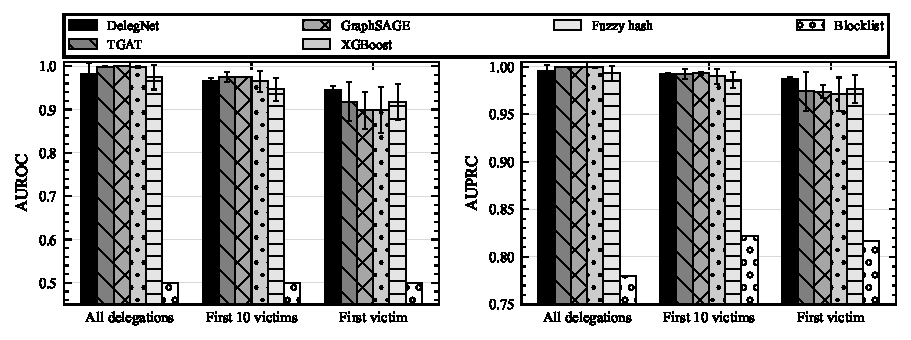
\includegraphics[width=0.4\textwidth]{fig_zeroday_slices}
\caption{Zero-day AUROC (left) and AUPRC (right) per evidence slice; bars show the mean over three seeds and whiskers one standard deviation. The blocklist is at chance on every slice. \dn{} has the highest mean on a contract's first victim and the smallest seed variance there.}
\label{fig:zeroday}
\end{figure}

\begin{figure}[t]
\centering
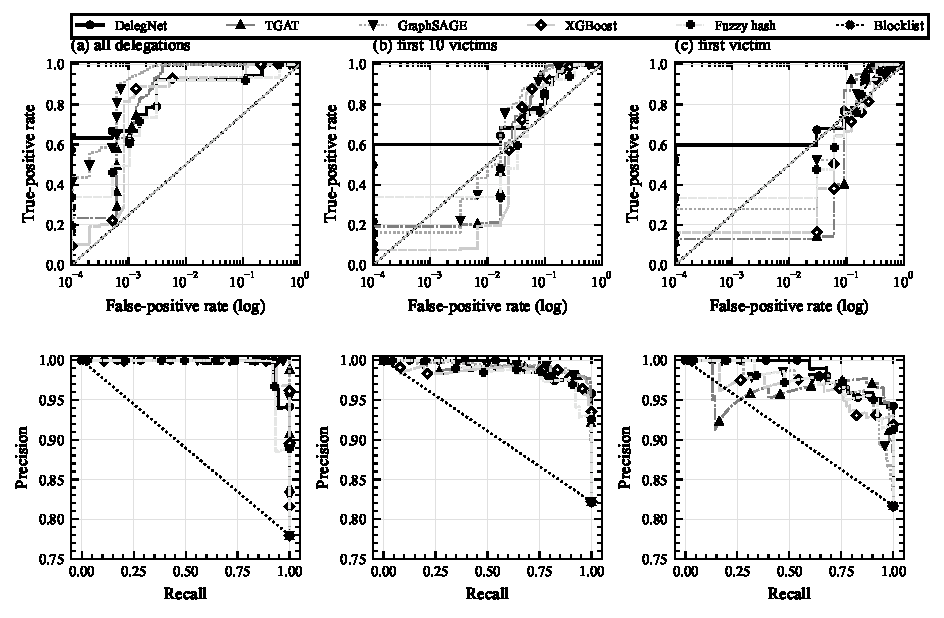
\includegraphics[width=0.4\textwidth]{fig_roc_pr}
\caption{ROC curves on a logarithmic false-positive axis (top) and precision--recall curves (bottom) for (a)~all delegations, (b)~the first ten victims and (c)~the first victim of each unseen contract, pooled over seeds.}
\label{fig:rocpr}
\end{figure}

Three findings stand out. First, the blocklist is at chance on every slice: an exact-match defence offers no protection against a new family, even when matching canonical rather than raw code. Second, on the full test population the temporal graph networks attain the highest AUROC ($0.999$) and \dn{} attains $0.982$. The graph models' advantage on this slice comes from sibling evidence: most test delegations belong to large campaigns whose earlier victims have already been drained by the time later victims delegate, which is visible to behavioural models but irrelevant to a code-based score. Third, on the \emph{first victim} of each new contract---where no sibling evidence exists and a detector must recognise the attack from what the contract is---\dn{} attains the highest AUROC ($0.946\pm0.009$), ahead of TGAT ($0.918$), fuzzy hashing ($0.918$), XGBoost ($0.899$) and GraphSAGE ($0.898$), with a seed standard deviation four to six times smaller than that of any learned baseline. Averaging three seeds raises \dn{}'s first-victim AUROC to $0.956$.

\paragraph{Score distributions} Fig.~\ref{fig:scores} shows why the code-based score generalises. On the first ten victims of unseen contracts, \dn{}'s malicious scores have interquartile range $[0.581, 0.662]$ and its benign scores $[0.413, 0.505]$; the ranges do not overlap, and the medians ($0.629$ and $0.459$) lie on either side of the indifference point $0.5$; the separation is produced by a contract's resemblance to theft code relative to wallet code, not by behaviour.

\begin{figure}[t]
\centering
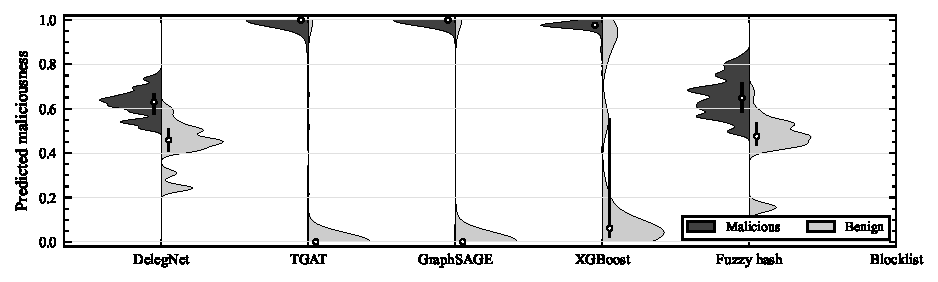
\includegraphics[width=0.4\textwidth]{fig_score_distributions}
\caption{Score distributions on the first ten victims of unseen contracts: malicious (dark, left half) and benign (light, right half) per method, with interquartile bars and medians.}
\label{fig:scores}
\end{figure}

\subsection{Effect of available evidence}
\label{sec:res-history}
Fig.~\ref{fig:history} resolves detection by the position of a delegation among its contract's victims. Behavioural models improve steeply as evidence accumulates: TGAT rises from $0.918$ on the first victim to $0.980$ for victims 2--10 and $1.000$ beyond the tenth, and GraphSAGE from $0.898$ to $1.000$. \dn{} is comparatively flat ($0.946$, $0.969$, $0.990$, $0.981$), because its decision does not depend on how many earlier victims have been drained. The two families of detectors are therefore strongest at opposite ends of a campaign. The first victims of a new campaign are, from a defender's perspective, the ones that matter most, since every later victim can in principle be protected by information about earlier ones; it is on these that \dn{} leads. The support panel of Fig.~\ref{fig:history} also explains why aggregate metrics favour behavioural models: per seed there are only $60$ first victims ($49$ malicious, $11$ benign), but $11{,}106$ delegations beyond the hundredth.

\begin{figure}[t]
\centering
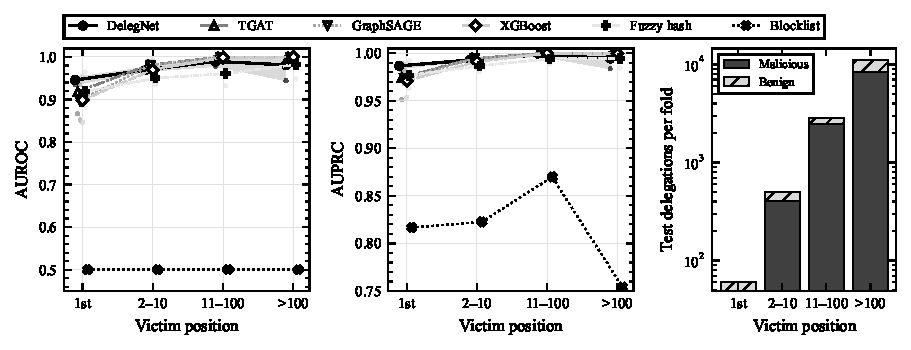
\includegraphics[width=0.4\textwidth]{fig_history_buckets}
\caption{Detection by evidence available at decision time. Left and centre: AUROC and AUPRC by the delegation's position among its contract's victims (mean line, per-seed points, \dn{}'s seed range shaded). Right: test support per bucket (malicious dark, benign hatched).}
\label{fig:history}
\end{figure}

\subsection{Robustness to code disguise}
\label{sec:res-disguise}
Fig.~\ref{fig:disguise} examines what happens when attackers re-deploy their contracts as semantics-preserving mutants. Panel~(b) shows the mechanism of failure for raw code matching: the four-gram similarity between a malicious contract and its mutant decays from $0.766$ at strength $0.25$ to $0.678$, $0.551$, $0.367$, $0.252$ and $0.192$ at strengths $0.5$ to $4$, uniformly across all $60$ contracts. Panel~(c) shows that the canonical form removes it: mean similarity stays at $0.999$--$1.000$ at every strength, and panel~(d) shows that this holds for each contract individually, with every point on the upper boundary regardless of its raw similarity.

The consequence for detection is shown in panel~(a). At the fixed operating threshold, fuzzy hashing's recall falls from $0.981$ to $0.822$ ($\sigma{=}0.5$), $0.579$ ($\sigma{=}1$) and $0.333$ ($\sigma{\ge}2$), whereas \dn{} remains at $0.984$ at every strength. Fuzzy hashing's AUROC is largely preserved ($0.991$), because mutation lowers malicious and benign similarities alike, but its scores collapse towards the indifference point, below any threshold set on clean data. A deployed fuzzy-hash detector would silently stop alerting. Detectors that do not read bytecode---the graph networks and the behavioural features of XGBoost---are unaffected by disguise, but, as the next experiment shows, are exposed to behavioural manipulation instead.

\begin{figure}[t]
\centering
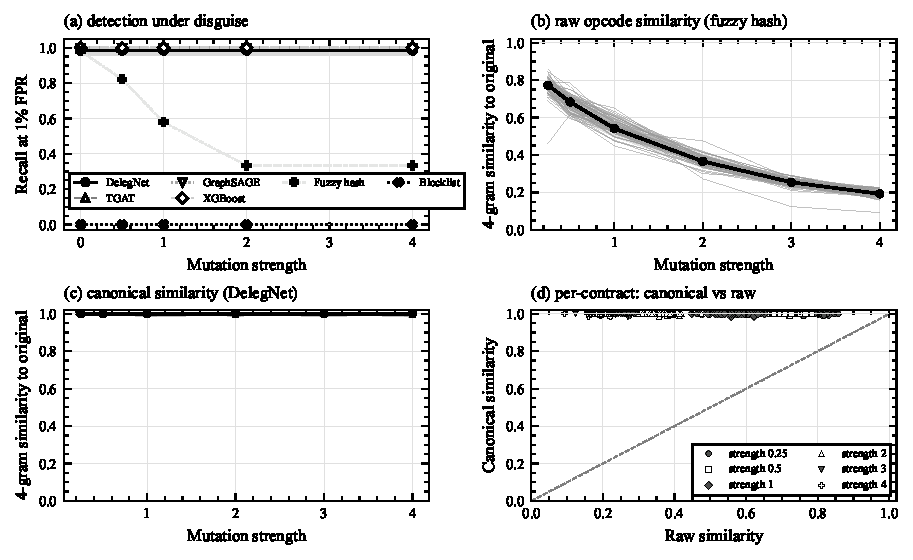
\includegraphics[width=0.4\textwidth]{fig_code_disguise}
\caption{Code disguise. (a)~Recall at 1\% FPR as mutation strength grows. (b)~Raw opcode four-gram similarity between each of 60 malicious contracts and its mutant (thin lines), with median, interquartile and 10--90\% bands. (c)~The same for \dn{}'s canonical form. (d)~Per-contract canonical versus raw similarity at six strengths.}
\label{fig:disguise}
\end{figure}

\subsection{Robustness to adaptive attackers}
\label{sec:res-evasion}
Table~\ref{tab:evasion} and Figs.~\ref{fig:evasion}--\ref{fig:evasion-prof} report the five-attack suite.

\begin{table}[t]
\centering
\caption{Recall at the clean-data 1\% FPR threshold under adaptive attacks (mean over three seeds; last zero-day fold of each seed). Attacks modify only attacker-controlled inputs of malicious delegations.}
\label{tab:evasion}
\footnotesize
\setlength{\tabcolsep}{2.4pt}
\begin{tabular}{lcccccc}
\toprule
Method & None & Self-sub. & Fresh spons. & Fresh contr. & Disguise & Combined \\
\midrule
Blocklist & 0.000 & 0.000 & 0.000 & 0.000 & 0.000 & 0.000 \\
Fuzzy hash & 0.981 & 0.981 & 0.981 & 0.981 & 0.333 & 0.333 \\
XGBoost & 1.000 & 0.666 & 0.667 & 1.000 & 1.000 & 0.667 \\
GraphSAGE & 1.000 & 0.548 & 1.000 & 1.000 & 1.000 & 0.229 \\
TGAT & 1.000 & 0.450 & 0.967 & 1.000 & 1.000 & 0.228 \\
\textbf{\dn{}} & \textbf{0.984} & \textbf{0.984} & \textbf{0.984} & \textbf{0.984} & \textbf{0.984} & \textbf{0.984} \\
\bottomrule
\end{tabular}
\end{table}

\begin{figure}[t]
\centering
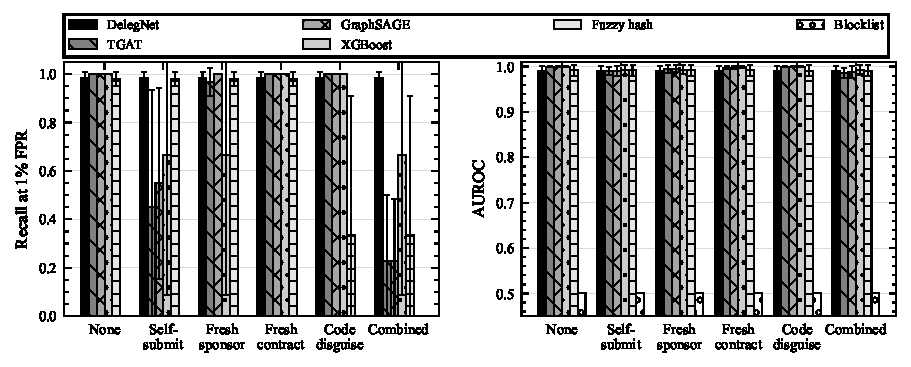
\includegraphics[width=0.4\textwidth]{fig_evasion_suite}
\caption{Adaptive-adversary suite: recall at the clean-data 1\% FPR threshold (left) and AUROC (right) for every method under each attack; whiskers show one standard deviation over seeds.}
\label{fig:evasion}
\end{figure}

\begin{figure}[t]
\centering
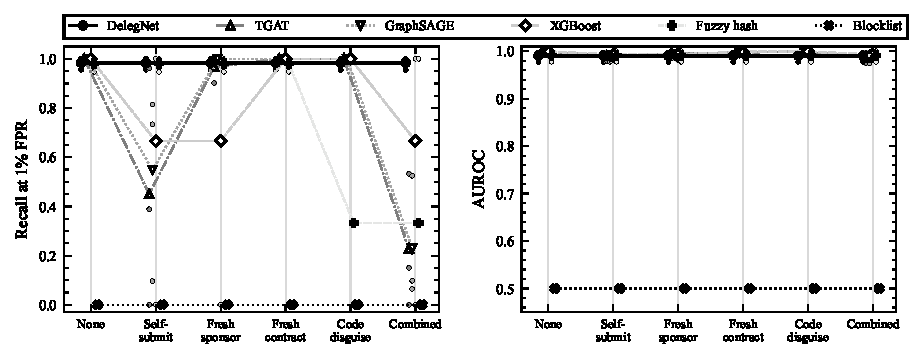
\includegraphics[width=0.4\textwidth]{fig_evasion_profiles}
\caption{Attack profiles: each line traces a method's mean recall (left) and AUROC (right) across attacks, with per-seed points. \dn{}'s profile is flat; behavioural detectors dip under self-submission and the combined attack.}
\label{fig:evasion-prof}
\end{figure}

\paragraph{Behavioural evasion} A single, costless change---submitting the authorization from the victim's own account instead of through a sponsor---reduces TGAT's recall from $1.000$ to $0.450$, GraphSAGE's to $0.548$ and XGBoost's to $0.666$. The models learned that sponsored, batched submission is characteristic of current campaigns. The feature is genuinely predictive on present data and entirely under the attacker's control. A fresh sponsor per victim primarily affects XGBoost ($0.667$), whose features include sponsor breadth and funding. The combined attack reduces both graph networks to $0.23$ recall: more than three quarters of malicious delegations pass undetected at the operating point. The graph networks' AUROC degrades only modestly ($0.986$--$0.990$), which shows that the attacks shift malicious scores downward across the board rather than scrambling their order. In deployment, however, a detector must commit to a threshold before it knows an attack is under way, and at that threshold the shift is decisive.

\paragraph{\dn{}} \dn{}'s recall is $0.984$ under every attack, identical to its clean-data recall, with AUROC $0.991$ throughout. This invariance follows from the design rather than from tuning: the score depends only on the delegate's canonical code, the behavioural attacks change nothing that it reads, and the disguise attack changes nothing that survives canonicalisation. The only way to evade \dn{} is to change what the contract does, and doing so means writing a new theft mechanism rather than re-using one.

\subsection{Screening before signing}
\label{sec:res-presig}
Because two thirds of thefts complete in the authorization's own block, protection must occur when the wallet asks the user to sign. Table~\ref{tab:presig} and Fig.~\ref{fig:presig} evaluate every method at that moment, when the signer and delegate are known but the sponsor is not.

\begin{table}[t]
\centering
\caption{Pre-signature screening (mean $\pm$ std over seeds): AUROC, recall and benign false-alarm rate at the clean-data operating threshold.}
\label{tab:presig}
\footnotesize
\setlength{\tabcolsep}{3.5pt}
\begin{tabular}{lccc}
\toprule
Method & AUROC & Recall & False alarms \\
\midrule
Blocklist & $0.500{\pm}.000$ & $0.000{\pm}.000$ & $0.000{\pm}.000$ \\
Fuzzy hash & $0.992{\pm}.012$ & $0.981{\pm}.029$ & $\mathbf{0.002}{\pm}.003$ \\
XGBoost & $\mathbf{0.999}{\pm}.001$ & $0.666{\pm}.576$ & $0.003{\pm}.005$ \\
GraphSAGE & $0.959{\pm}.043$ & $0.535{\pm}.329$ & $0.034{\pm}.030$ \\
TGAT & $0.931{\pm}.109$ & $0.501{\pm}.497$ & $0.189{\pm}.185$ \\
\textbf{\dn{}} & $0.991{\pm}.011$ & $\mathbf{0.984}{\pm}.025$ & $\mathbf{0.002}{\pm}.003$ \\
\bottomrule
\end{tabular}
\end{table}

\begin{figure}[t]
\centering
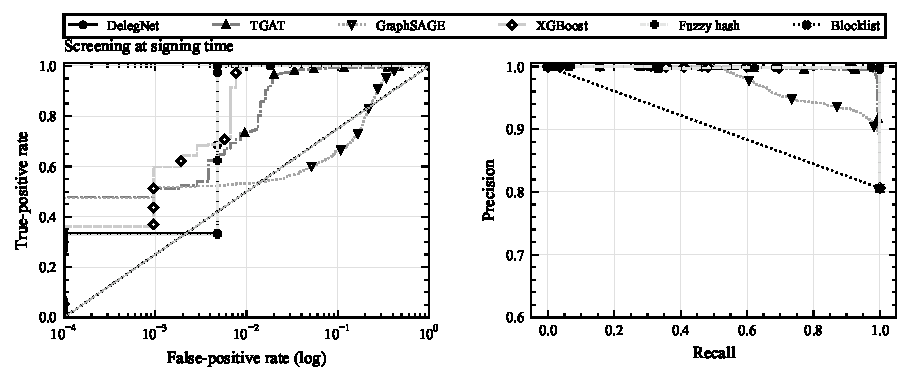
\includegraphics[width=0.4\textwidth]{fig_presignature}
\caption{Screening at signing time: ROC curves on a logarithmic false-positive axis (left) and precision--recall curves (right), seed~0, last zero-day fold.}
\label{fig:presig}
\end{figure}

\dn{} detects $98.4\%$ of malicious delegation requests with a false-alarm rate of $0.16\%$---roughly one unnecessary warning per $600$ benign delegations---and is stable across seeds. The behavioural detectors lose the evidence they rely on: without the sponsor and the authorization event, TGAT's recall falls to $0.501$ with an $18.9\%$ false-alarm rate, and GraphSAGE's to $0.535$ at $3.4\%$. XGBoost ranks pre-signature requests well (AUROC $0.999$, since it also reads code idioms), but its recall at the operating threshold varies between seeds from $0$ to $1$ ($0.666\pm0.576$). Its threshold, calibrated on post-inclusion behaviour, does not transfer to the pre-signature distribution of its inputs. Fuzzy hashing matches \dn{} at signing time on clean code, but it inherits the $0.333$ recall of Section~\ref{sec:res-disguise} as soon as attackers mutate their bytecode.

\subsection{Post-inclusion monitoring}
\label{sec:res-monitor}
Table~\ref{tab:monitor} evaluates a monitoring deployment that scores delegations at checkpoints after inclusion and blocks further outflows on alert.

\begin{table}[t]
\centering
\caption{Post-inclusion monitoring (last zero-day fold, mean over seeds): share of malicious delegations alerted, share alerted before their first theft, share of stolen value leaving after the alert, benign false-alarm rate, and AUROC at inclusion and two hours later.}
\label{tab:monitor}
\footnotesize
\setlength{\tabcolsep}{2.2pt}
\begin{tabular}{lcccccc}
\toprule
Method & Alerted & Pre-theft & Value saved & False al. & AUC@0s & AUC@2h \\
\midrule
Blocklist & 0.000 & 0.000 & 0.000 & 0.000 & 0.500 & 0.500 \\
Fuzzy hash & 0.981 & 0.994 & 0.999 & 0.002 & 0.992 & 0.992 \\
XGBoost & 1.000 & 1.000 & 1.000 & 0.007 & 1.000 & 1.000 \\
GraphSAGE & 1.000 & 1.000 & 1.000 & 0.011 & 1.000 & 1.000 \\
TGAT & 1.000 & 1.000 & 1.000 & 0.023 & 1.000 & 1.000 \\
\textbf{\dn{}} & 0.984 & 0.995 & 0.999 & \textbf{0.002} & 0.991 & 0.991 \\
\bottomrule
\end{tabular}
\end{table}

All learned detectors alert on nearly every malicious delegation at the moment of inclusion and before its first theft is recorded. \dn{} does so with the lowest false-alarm rate ($0.16\%$, against $0.7$--$2.3\%$ for the behavioural models), which matters at the scale of $634{,}828$ delegations in two months. The pre-theft figure must, however, be read alongside the dataset statistics: $67.7\%$ of thefts occur within the authorization's own block, typically in the very transaction that carries it, so an alert raised after inclusion cannot stop them. Monitoring is therefore a complement to, not a substitute for, screening before signing, where \dn{} is the only reliable method.

\subsection{Contract-level reliability and statistical significance}
\label{sec:res-contract}
Fig.~\ref{fig:contract} examines the $60$ held-out contracts individually. The heatmap shows each contract's mean score over its first ten victims, and the violins show bootstrap distributions of contract-level AUROC. \dn{} separates malicious from benign contracts with AUROC $0.952$ [0.869, 1.000], compared with $0.987$ [0.956, 1.000] for TGAT, $0.983$ for GraphSAGE, $0.964$ for fuzzy hashing and $0.891$ [0.740, 1.000] for XGBoost. Table~\ref{tab:sig} reports paired bootstrap comparisons on identical delegations. On the first victim and the first ten victims, \dn{}'s differences to every learned baseline lie within bootstrap uncertainty, a consequence of having $60$ first victims per seed and only $11$ labelled benign contracts. On the full population the graph networks are significantly more accurate, by $0.017$ AUROC, reflecting their use of sibling evidence on later victims. Against the blocklist, \dn{} is better by $0.45$--$0.48$ AUROC on every slice ($p<0.001$). The decisive differences in favour of \dn{} are those of Sections~\ref{sec:res-disguise}--\ref{sec:res-presig}: a recall of $0.984$ against $0.228$--$0.333$ under attack, and against $0.50$--$0.54$ for graph networks before signing.

\begin{figure}[t]
\centering
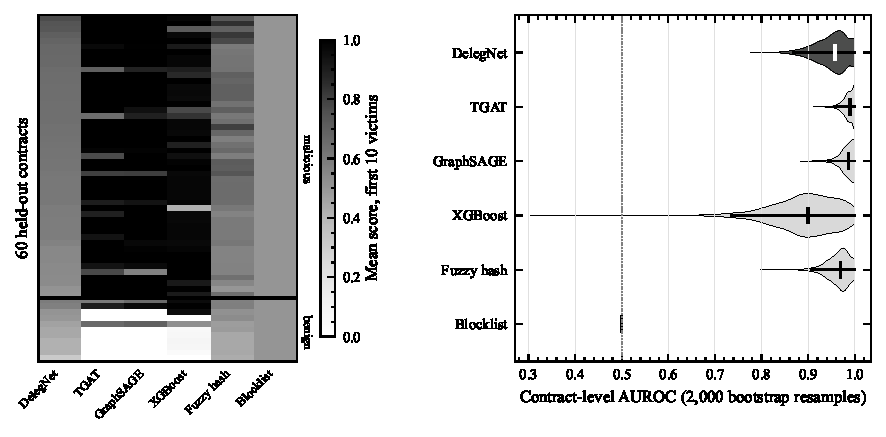
\includegraphics[width=0.4\textwidth]{fig_contract_level}
\caption{Contract-level analysis. Left: mean score over the first ten victims for every held-out contract (rows; malicious above the line, benign below) and method (columns). Right: contract-level AUROC over 2{,}000 bootstrap resamples of contracts, with 95\% intervals and medians.}
\label{fig:contract}
\end{figure}

\begin{table}[t]
\centering
\caption{Paired bootstrap difference in AUROC (\dn{} minus baseline), mean over seeds, with 95\% interval.}
\label{tab:sig}
\footnotesize
\setlength{\tabcolsep}{3pt}
\begin{tabular}{lccc}
\toprule
Baseline & All & First 10 & First victim \\
\midrule
Blocklist & $+0.482$ [0.481, 0.484] & $+0.467$ [0.448, 0.482] & $+0.446$ [0.360, 0.500] \\
Fuzzy hash & $+0.008$ [0.005, 0.010] & $+0.020$ [0.006, 0.034] & $+0.027$ [$-0.023$, 0.087] \\
XGBoost & $-0.016$ [$-0.018$, $-0.014$] & $+0.002$ [$-0.019$, 0.023] & $+0.045$ [$-0.039$, 0.143] \\
GraphSAGE & $-0.017$ [$-0.019$, $-0.016$] & $-0.008$ [$-0.024$, 0.009] & $+0.048$ [$-0.032$, 0.148] \\
TGAT & $-0.017$ [$-0.019$, $-0.015$] & $-0.008$ [$-0.027$, 0.012] & $+0.029$ [$-0.065$, 0.141] \\
\bottomrule
\end{tabular}
\end{table}

\subsection{Validity audit}
\label{sec:res-validity}
Fig.~\ref{fig:leak} reports the label-permutation and shuffled-label checks. For every learned method the observed test AUROC lies far outside the null distribution obtained by permuting test labels $1{,}000$ times (null mean $0.500$, 97.5th percentile $\le 0.558$, permutation $p=0.001$, the smallest attainable), so all reported separations are statistically real. When XGBoost is retrained on class-balanced data with shuffled labels, its test AUROC falls to $0.38\pm0.10$ on all delegations and $0.44\pm0.09$ on first victims: no path in the pipeline carries label information when the training labels carry none. Train, validation and test AUROC for the final fold are $1.000$, $1.000$ and $0.997$ for \dn{}, $1.000$, $1.000$ and $0.999$ for TGAT and GraphSAGE, and $1.000$, $1.000$ and $0.999$ for XGBoost; no method exhibits a train--test gap indicative of overfitting.

\begin{figure}[t]
\centering
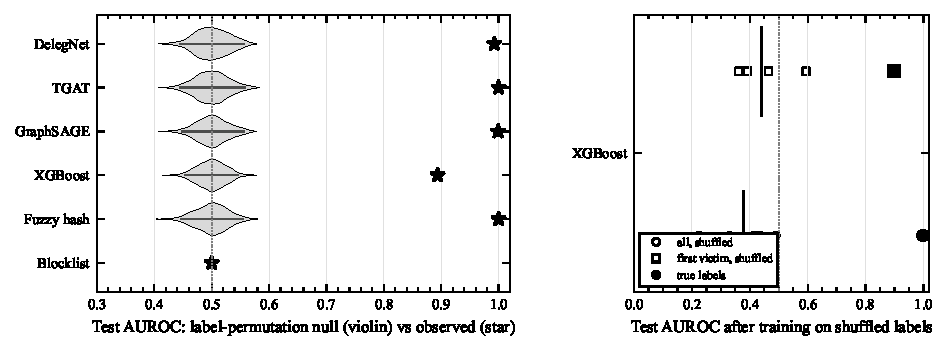
\includegraphics[width=0.4\textwidth]{fig_leakage_audit}
\caption{Validity audit. Left: null distributions of test AUROC under 1{,}000 permutations of test labels (violins, 95\% bars) versus observed AUROC (stars). Right: test AUROC after retraining on class-balanced shuffled labels (open markers; bars give the mean) versus training on true labels (filled).}
\label{fig:leak}
\end{figure}

\subsection{Summary of capabilities}
Fig.~\ref{fig:capability} condenses the evaluation. The behavioural graph networks are the most accurate detectors when attackers behave as they did in the observed campaigns and evidence about earlier victims is available. Every capability that depends on resisting an adaptive attacker or acting before signing, however, is held by \dn{} alone: first-victim detection ($0.946$), recall under the combined attack ($0.984$), under self-submission ($0.984$), under code disguise ($0.984$) and before signing ($0.984$).

\begin{figure}[t]
\centering
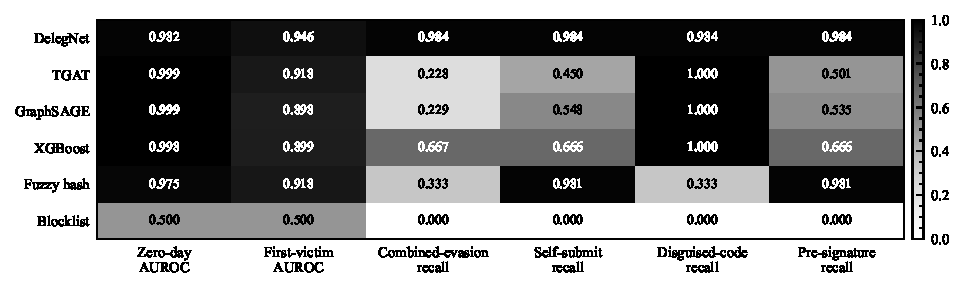
\includegraphics[width=0.4\textwidth]{fig_capability_matrix}
\caption{Capability matrix: zero-day AUROC, first-victim AUROC, and recall at 1\% FPR under the combined attack, self-submission, code disguise ($\sigma{=}4$) and before signing. Bold marks the best value per column.}
\label{fig:capability}
\end{figure}

\section{Discussion}
\label{sec:discussion}

\subsection{Why behavioural detectors fail against adaptive attackers}
The graph networks learn exactly what they are trained to learn: in the observed campaigns, malicious delegations are submitted by sponsors in batches, from accounts funded by earlier drains, to contracts whose earlier victims have already been swept. These regularities are statistically strong---they yield an AUROC of $0.999$ on unseen families---but they are properties of the attackers' current \emph{operations}, not of theft. Each can be removed for the cost of a few transactions: a leaked-key attacker can sign and submit from the victim's account, fund gas through a fresh path, or deploy one contract per victim. Our suite shows that such changes leave the ranking of graph models largely intact, yet move malicious scores below any threshold calibrated on historical behaviour. The general lesson for security applications of temporal graph learning is that high accuracy on behaviour-rich historical data says little about robustness when the behaviour is attacker-chosen. Evaluations should include attacks on the features a model actually relies on.

\subsection{Why canonical code patterns are robust}
A theft mechanism must exist in the delegate's code: value has to be forwarded to an attacker-controlled destination, or an attacker-controlled caller has to be granted arbitrary execution. The cheapest way to field a new campaign is to copy an existing mechanism and vary only its surface---addresses, filler instructions, equivalent opcodes, appended data. \dn{}'s canonicalisation is designed around precisely this economics. It removes, by construction, every transformation in the class $\mathcal{M}$, so copying no longer evades detection, and an attacker who wants to escape the memory must implement theft differently, which is substantially more expensive than re-deploying a template. The memory's family exclusion ensures that what \dn{} learns is resemblance to \emph{other} known mechanisms, which is the property needed for new families. That first-victim detection is \dn{}'s strongest accuracy slice is consistent with this interpretation.

\subsection{Deployment}
\paragraph{Wallets} \dn{} needs only the delegate address of a signature request: the wallet retrieves the code, canonicalises it and scores it against a memory distributed as a list of four-gram sets. At a 1\% validation false-positive operating point it warns on $98.4\%$ of malicious requests while interrupting about one in $600$ benign ones, and each warning cites the specific known contract the request resembles.
\paragraph{Monitoring services} Explorers and security providers can run \dn{} alongside behavioural detectors. The latter are more accurate once a campaign has accumulated victims, while \dn{} covers the first victims, disguised re-deployments and attackers who abandon sponsored submission. A disagreement between the two is itself informative: a high code score with a low behavioural score is the signature of an attacker who has changed operations but not mechanism.
\paragraph{Memory maintenance} New confirmed families are added to the memory without retraining. Because labels can be derived automatically from outcomes (Section~\ref{sec:data}), the memory can be refreshed continuously, with human review reserved for borderline contracts.

\subsection{What an attacker can still do}
\dn{}'s guarantee covers the transformation class $\mathcal{M}$. Attackers could move beyond it, at higher cost:
\begin{itemize}
\item \emph{Semantic obfuscation}: opaque predicates, computed jump targets, or arithmetic encoding of the attacker address. Computed jump targets defeat static reachability; this is a known limit of static analysis that symbolic execution of the dispatcher would address.
\item \emph{Indirection}: a minimal proxy that \texttt{DELEGATECALL}s into separately deployed logic. Our idioms flag delegate calls to calldata- or storage-derived targets, and resolving the implementation and canonicalising it as well is a direct extension.
\item \emph{Novel mechanisms}: a genuinely new theft mechanism has no close memory match and receives an intermediate score. This is the regime where behavioural evidence, accumulated over the first victims, becomes valuable.
\end{itemize}
Each of these raises the attacker's cost relative to today's practice of re-deploying copied templates.

\subsection{Limitations}
\paragraph{Benign coverage} Our labelling rules require at least five delegators and sustained owner activity before a contract is labelled benign, which yields $11$ benign contracts in $9$ families. This is conservative---it avoids labelling as benign a contract whose victims simply have not been drained yet---but it bounds the precision of contract-level estimates, as the bootstrap intervals of Table~\ref{tab:sig} show. Curated lists of official wallet implementations would enlarge the benign set.
\paragraph{Assets and chains} Activity was collected for native ether, including internal transfers, but not for ERC-20 tokens, because free endpoints do not serve historical logs at the required scale. Drainers that steal only tokens are therefore labelled from their ether behaviour alone. The study covers Ethereum; other chains that adopted EIP-7702 lack free historical trace access, and per-address explorer data would enable a cross-chain evaluation.
\paragraph{Sampling} Activity was collected for a per-contract stratified sample of up to $1{,}000$ delegators. The full authorization scan is released, so that complete histories can be added with commercial data access.
\paragraph{Window} The window covers the first two months after activation, when sweepers dominated. As the mechanism matures, the balance between benign and malicious delegations, and the attackers' operations, will change. Continuous re-evaluation under the zero-day protocol is the appropriate response.

\subsection{Threats to validity}
\emph{Internal}: labels are derived from outcomes with fixed rules, and mislabelled contracts would affect every method equally. The rules are reported in full, the evidence behind every label is released, and the independent cross-check found no benign contract associated with a known scam address. \emph{Construct}: AUROC and fixed-false-positive recall measure ranking and operating-point behaviour respectively, and we report both, together with contract-level aggregation to prevent large campaigns from dominating. \emph{External}: results depend on the attack mix of the observation window; the adaptive-adversary suite probes deviations from it, but only along the dimensions we modelled. \emph{Conclusion}: with $60$ first-victim contracts per seed, first-victim differences between learned methods are within bootstrap uncertainty, and we draw no conclusion from them beyond \dn{}'s consistently high and stable performance on that slice.

\subsection{Ethics and data release}
All data are public ledger records. Addresses are pseudonymous, and we release no off-chain identities, link no addresses to individuals, and publish no information not already present on chain. The dataset documents attacker infrastructure that is already publicly visible, and its release supports defenders more than attackers, who already possess it. The canonicaliser and mutator describe transformations attackers already apply; publishing them strengthens defences without enabling new attacks. The dataset is accompanied by a data card describing collection, labelling rules, known limitations and intended use.


\section{Conclusion}
\label{sec:conclusion}
EIP-7702 converted account takeover into a one-signature operation, and attackers industrialised it within days. We assembled the first labelled dataset of real EIP-7702 delegations and evaluated detectors under the conditions a defence actually faces: unseen contract families, adaptive attackers and decisions before signing. Temporal graph detectors are the most accurate on non-adversarial data but rely on behaviour that attackers control, and they lose most of their recall under simple, cheap behavioural changes. Code matching is behaviour-independent, but on raw bytecode it is defeated by mutation. \dn{}'s canonical code-pattern recognition removes the transformations attackers apply to copied contracts and therefore keeps a recall of $0.984$ under every attack we evaluated, detects a family's first victim best, and screens authorizations before they are signed with a negligible false-alarm rate. We release the dataset, protocol and implementation to support further work on this rapidly evolving threat.

\section*{Data and Code Availability}
The dataset (authorizations with recovered signers, delegate bytecode, labels with evidence, account transfer histories and zero-day fold assignments) is released under CC BY 4.0 at [DOI to be added on deposit]. The complete pipeline, from raw chain data to every table and figure, is available at [repository URL to be added].

\balance
\bibliographystyle{IEEEtran}
\bibliography{references}

\end{document}
